\documentclass{article}
\usepackage{graphicx}
\usepackage{amsthm}
\usepackage{amsfonts}
\usepackage{amsmath}
\usepackage{amssymb}
\usepackage{fullpage}
\usepackage[usenames]{color}
\usepackage{hyperref}
  \hypersetup{
    colorlinks = true,
    urlcolor = blue,       % color of external links using \href
    linkcolor= blue,       % color of internal links 
    citecolor= blue,       % color of links to bibliography
    filecolor= blue,        % color of file links
    }
    
\usepackage{listings}

\definecolor{dkgreen}{rgb}{0,0.6,0}
\definecolor{gray}{rgb}{0.5,0.5,0.5}
\definecolor{mauve}{rgb}{0.58,0,0.82}

\lstset{frame=tb,
  language=haskell,
  aboveskip=3mm,
  belowskip=3mm,
  showstringspaces=false,
  columns=flexible,
  basicstyle={\small\ttfamily},
  numbers=none,
  numberstyle=\tiny\color{gray},
  keywordstyle=\color{blue},
  commentstyle=\color{dkgreen},
  stringstyle=\color{mauve},
  breaklines=true,
  breakatwhitespace=true,
  tabsize=3
}

\theoremstyle{theorem} 
   \newtheorem{theorem}{Theorem}[section]
   \newtheorem{corollary}[theorem]{Corollary}
   \newtheorem{lemma}[theorem]{Lemma}
   \newtheorem{proposition}[theorem]{Proposition}
\theoremstyle{definition}
   \newtheorem{definition}[theorem]{Definition}
   \newtheorem{example}[theorem]{Example}
\theoremstyle{remark}    
  \newtheorem{remark}[theorem]{Remark}


\title{CPSC-354 Report}
\author{Michael Masakayan  \\ Chapman University}

\date{\today}

\begin{document}

\maketitle

\begin{abstract}
Short  summary of purpose and content.  
\end{abstract}
\tableofcontents


\section{Introduction}\label{intro}

~\ref{intro} My name is Michael Masakayan, I'm a 4th year computer science major. I transferred from Pasadena City College in 2020. I am interested in cyber security and although I won't be able to get a minor in it I plan on getting a few certificates this year. I enjoy playing video games and like watching movies


\section{Homework}\label{homework}

This section will contain your solutions to homework. 

\subsection{Week 1}
 Assignment 1: GCD. The program figures out the Greatest Common Divisor for any given two numbers using Euclid’s algorithm. 
\begin{enumerate}

\item Firstly you want to put the program into your IDE and run g++ -o assignment1 assignment.cpp
\item then type in ./assignment1.cpp
\item Once you run the program you type in the first number then you hit enter then you type in the second number and hit enter. It will then show you the GCD of the two numbers.
    \end{enumerate}
      I chose to use c++ because I am familiar with the language and it was easier for me to write the program in it. This assignment was mainly for us to get used to using LaTeX
\begin{lstlisting}
#include <iostream>
using namespace std;
int gcd(int n, int m) {
   if (m == 0)
   {
       return n;
   }
  
   else if(n>m)
   {
      gcd(m,n-m);
   }
   else if(n<m)
   {
      gcd(n,m-n);
   }
   return gcd(m, n % m);
}
int main() {
    int n,m;
    cout<<"type the number for the first argument of the GCD, then hit enter"<<'\n';
    cin>>n;
    cout<<"type the number for the first argument of the GCD,then hit enter"<<'\n';
    cin>>m;
   cout<<"GCD of "<< n <<" and "<< m <<" is "<< gcd(n, m);
   return 0;
}
\end{lstlisting}
\subsection{Week 2}
 Assignment 2: In this assignment we were tasked with creating a few recursiver functions in haskel that is  
  
\begin{enumerate}

\item select_evens
\item select_odds
\item member
\item append
\item revert
\item less_equal

Select evens will take a list and return a another list with only the even elements of the list in the argument. select_odds is meant to do what select even does but for the odds items in the list. Member, is meant to check a list if it has the given argument in it returning true if it contains it and false if it does not. The append method will combine two lists into one and return the combine list. Revert is meant to change the order of a list so that it will be backwards. And finaly less_equal is meant to check if a list is less than or equal to another list. 
\begin{enumerate}

\item Firstly you want to put the program into your IDE and run ghci
\item then type in  :load assignment2.hs
\item you can type the following  and they should give the results
   \begin{enumerate}

\item select_evens ["e","f","g","h","i"]--result ["f","h"]
\item 
\item select_odds ["e","f","g","h","i"]--result["f","h","i"]
\item 
\item member 3 [2,4,3]--result true member 3 [2,4,2]--result false
\item 
append [2,1] [3,1,2]
--result [2,3,1,1,2]
\item revert [5,6,7,8]
--result [8,7,6,5]
\item less_equal[1][2]
--result true
\item less_equal[3][2]
--result false

\end{enumerate}





I mainly had issue with less equal. I could not find the syntax for how to recursively go through more than one element lists. Most of them used the same type of recursion.


\begin{lstlisting}
{-let ezample_eveny =  ["a","b","c","d","e"] -}
{-yelect_eveny (z:zy) n =  z !!n if z !! n/2 == % 0 then b:a!! n 
-}
select_evens::  [a] -> [a]
select_evens [] = []
select_evens [x] = []
select_evens (x1:x2:xy) = x2:select_evens xy
-- selects all the odd elements in a list
select_odds ::  [a] -> [a]
select_odds [] = []
select_odds [x] = [x]
select_odds (x1:x2:xy) = x2:select_odds xy
-- member takes an int and a list and checks if the int is in the list

member:: Eq a=> a-> [a] -> Bool
member _ [] = False
member x (z:zs)=  (x `elem` zs) == True



-- combines two lists into one list
append ::  [a] -> [a] -> [a]
append [] xy = xy
append (z:zy) xy = z:append xy zy
-- reverses the order of a list
revert :: [a] -> [a]
revert xs = rev [] xs where
  rev :: [a] -> [a] -> [a] 
  rev acc    []  =       acc
  rev acc (x:xs) = rev (x:acc) xs
--compares the values of the lists
less_equal:: Ord a=> [a] -> [a] -> Bool
less_equal  [][] = True
less_equal [x][b] = (x>=b)
-- less_equal (x:xs) (b:bz) = x<b:less_equal xs bz



main::IO ()
main = print(append [1,2] [3,4,5])
-- print(less_equal [][])
-- print(select_odds ["a","b","c","d","e"])
-- print (revert [1,2,3])
\end{lstlisting}


\subsection{Week 6}
For homework 6 we were suppose to evaluate:
\begin{itemize}
\item ( \lambda exp .  \lambda two .  \lambda three . exp two three)
\item
\item  ( \lambda m. \lambda n. m n)
\item
\item  ( \lambda f. \lambda x. f (f x))
\item
\item  ( \lambda f. \lambda x. f (f (f x)))
\end{itemize}
\end{itemize}
From here we did a step by step simplifying the problem. We went over this class and there was a video teaching us on how we should do it. We also were suppose to go over our project outline and solitify what we will be doing for the final project

\begin{itemize}
\item =(( \lambda m. \lambda n. m n) ( \lambda f. \lambda x. f (f x)) ( \lambda f. \lambda x. f (f (f x))))
\item 
\item =(( \lambda m. \lambda n. m n) ( \lambda f. \lambda x. f (f x)) ( \lambda f2. \lambda x2. f2 (f2 (f2 x2))))
\item 
\item = (( ( \lambda f \lambda x. f (f x)) ( \lambda f2. \lambda x2. f2 (f2 (f2 x2)))))
\item 
\item =(( ( \lambda x. ( \lambda f2. \lambda x2. f2 (f2 (f2 x2) (( \lambda f2. \lambda x2. f2 (f2 (f2 x2) x)))
\item 
\item =(( ( \lambda x. ( \lambda f2. \lambda x2. f2 (f2 (f2 x2) (( \lambda x2. x (x (x x2))))
\item 
\item =(( ( \lambda x. \lambda x2. \lambda x2. x (x (x x2))(( \lambda x2. x(x (x x2))( \lambda x2. x( x(x x2)) x2))))
\item 
\item =(( ( \lambda x. \lambda x2. \lambda x2. x (x (x x2))( \lambda x2. x(x (x x2))(x (x (x x2))))))
\item 
\item =(( ( \lambda x. \lambda x2. \lambda x2. x (x (x x2))(x (x (x (x (x (x x2))))))))
\item 
\item =(( ( \lambda x. \lambda x2. x (x (x (x (x (x (x (x (x x2))))))))))
\end{itemize}
\end{enumerate}
We also had to do the excersices we had to do in class.I have attached the photo in latex and in the github if it dosn't load it should be hw6.jpg
\end{enumerate}
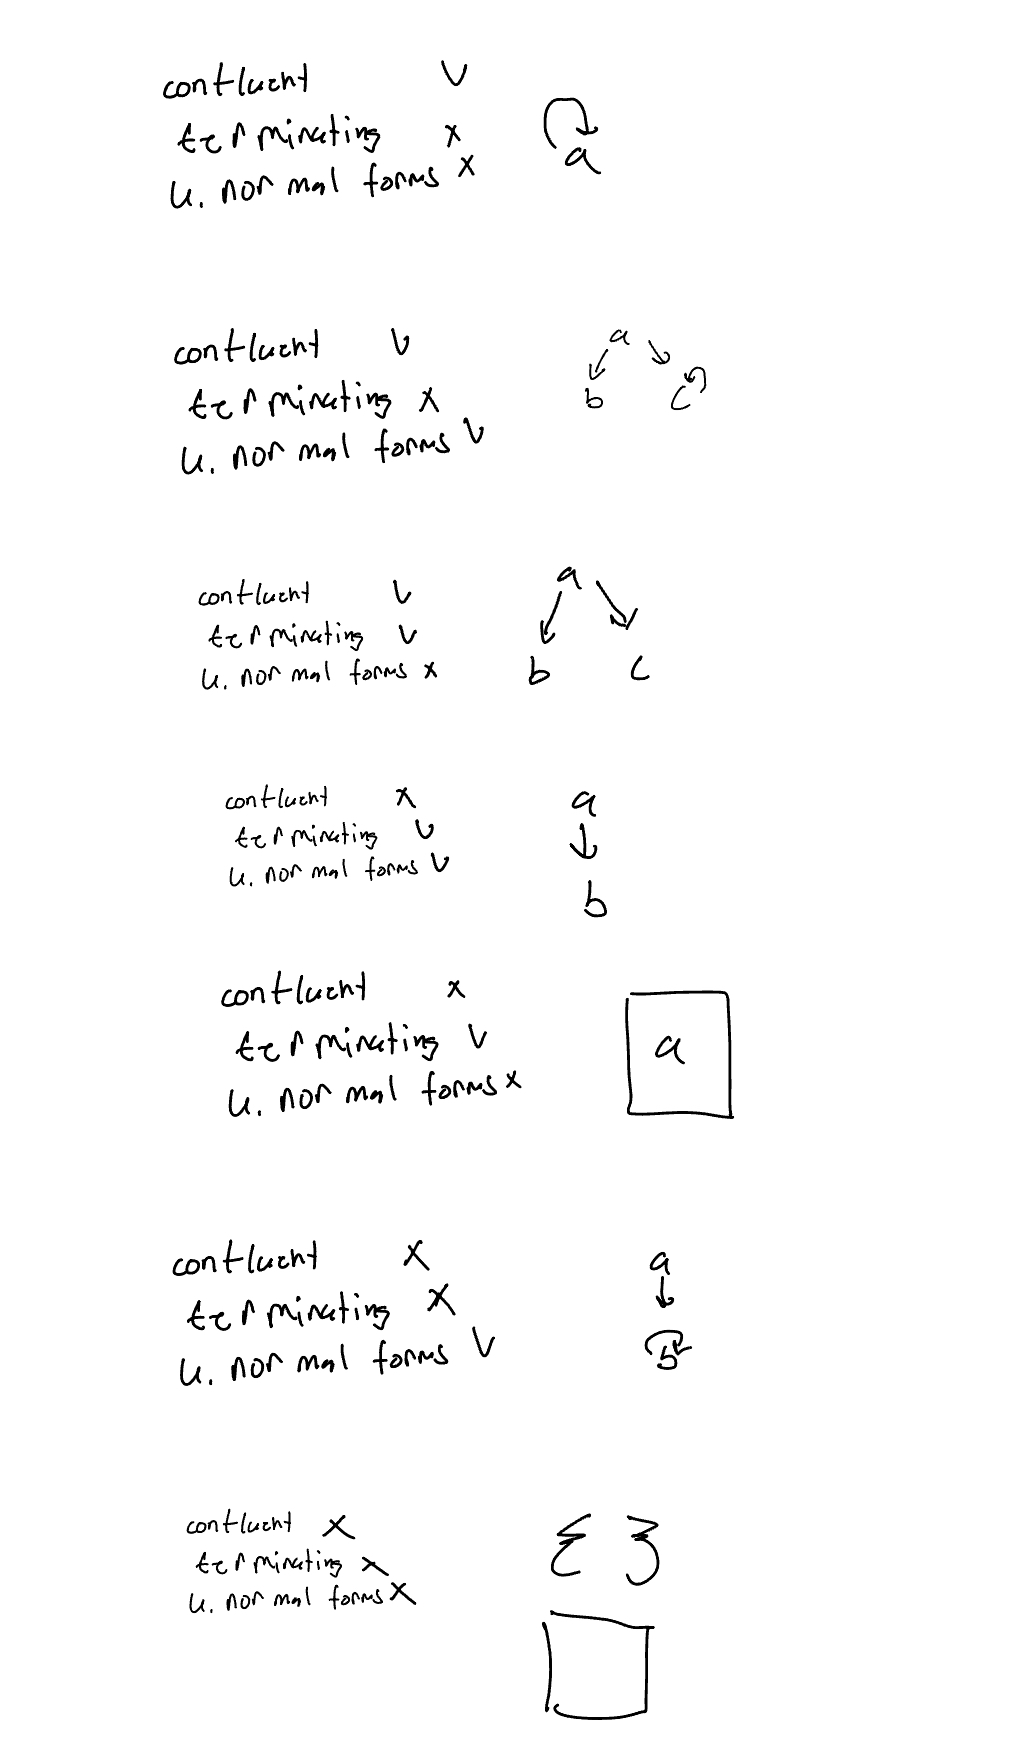
\includegraphics[scale=0.2]{hw6.jpg}
\subsection{Week 7}


2) If you have not done the evalCBN part of hw5, do it for this homework.
\begin{lstlisting}
`(\x.\y.x) y z`

evalCBN ((EApp  (EAbs (Id "x") (EVar (Id "x"))) (EApp (EAbs (Id "y") (EVar (Id "y"))) (EVar (Id "a")))))
== line 6
evalCBN (subst (Id "x" ) (EApp (EAbs (Id "y") (EVar (Id "y"))) (EVar (Id "a"))) (Evar (Id "x"))) 
== line 15
evalCBN (EApp (EAbs (Id "y") (EVar (Id "y"))) (EVar (Id "a")))
== line 6
evalCBN (subst (Id "y") (EVar (Id "a")) (EVar (Id "y")))
 == line 15
evalCBN (EVar ( Id "a"))
 == line 8
EVar (Id "a")

evalCBN (EApp (EAbs (Id "x") (EAbs (Id "y") (EVar (Id "x")))) (EVar (Id "y")) (EVar (Id "z"))) 
== line 6
evalCBN(subst (Id "x") (EAbs (Id "y") (EVar (Id "x"))) (EVar (Id "y")) (EVar (Id "z")))
 == line 15
evalCBN(EApp  (EAbs (Id "y") (EVar (Id "y"))) (EVar (Id "z")))
== line 6
evalCBN (subst (Id "y") (EVar (Id "z")) (EVar (Id "y")))
 == line 15
evalCBN (EVar (Id "z")) 
 == line 8
EVar (Id  "z")
\end{lstlisting}


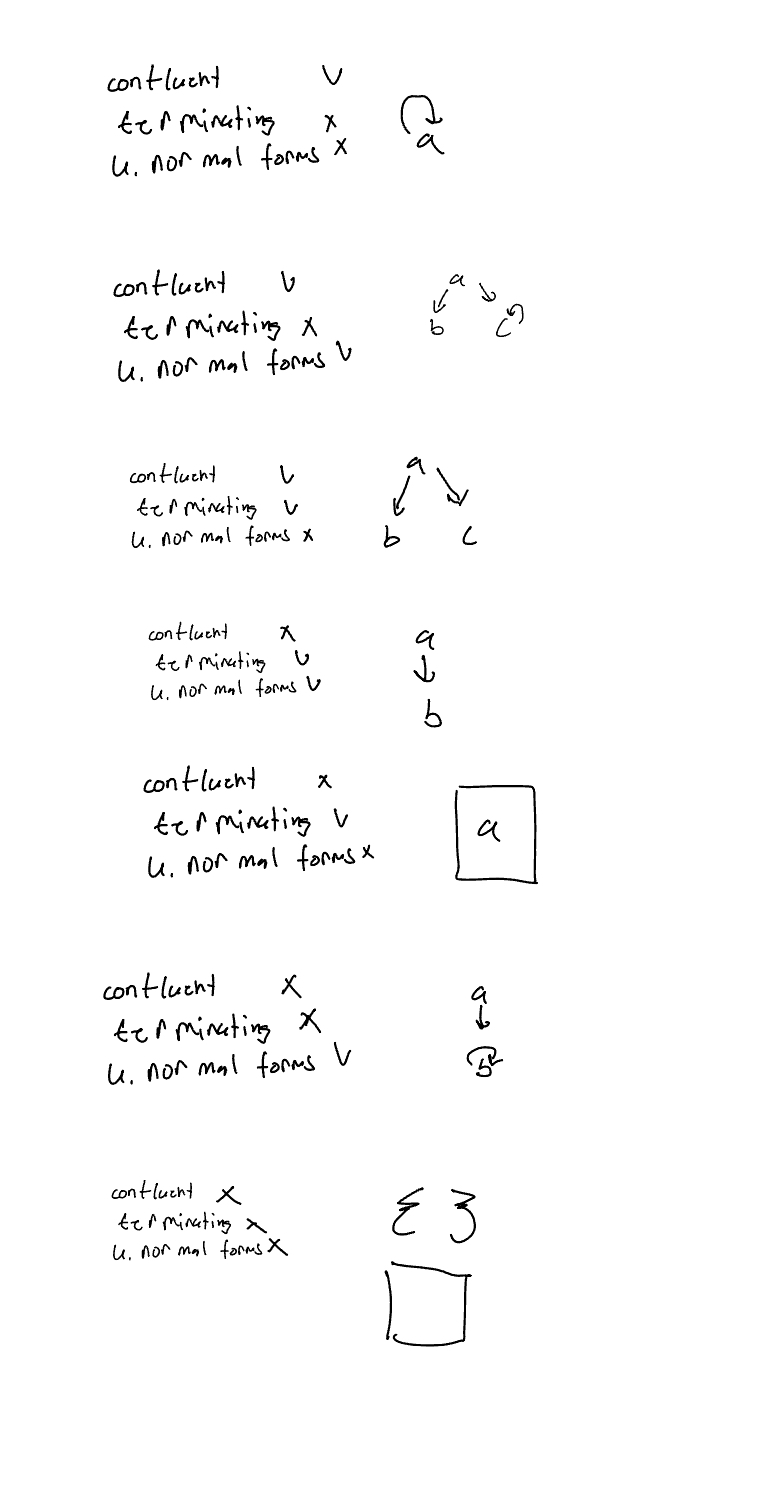
\includegraphics[scale=0.2]{hw7.2.jpg}
\item 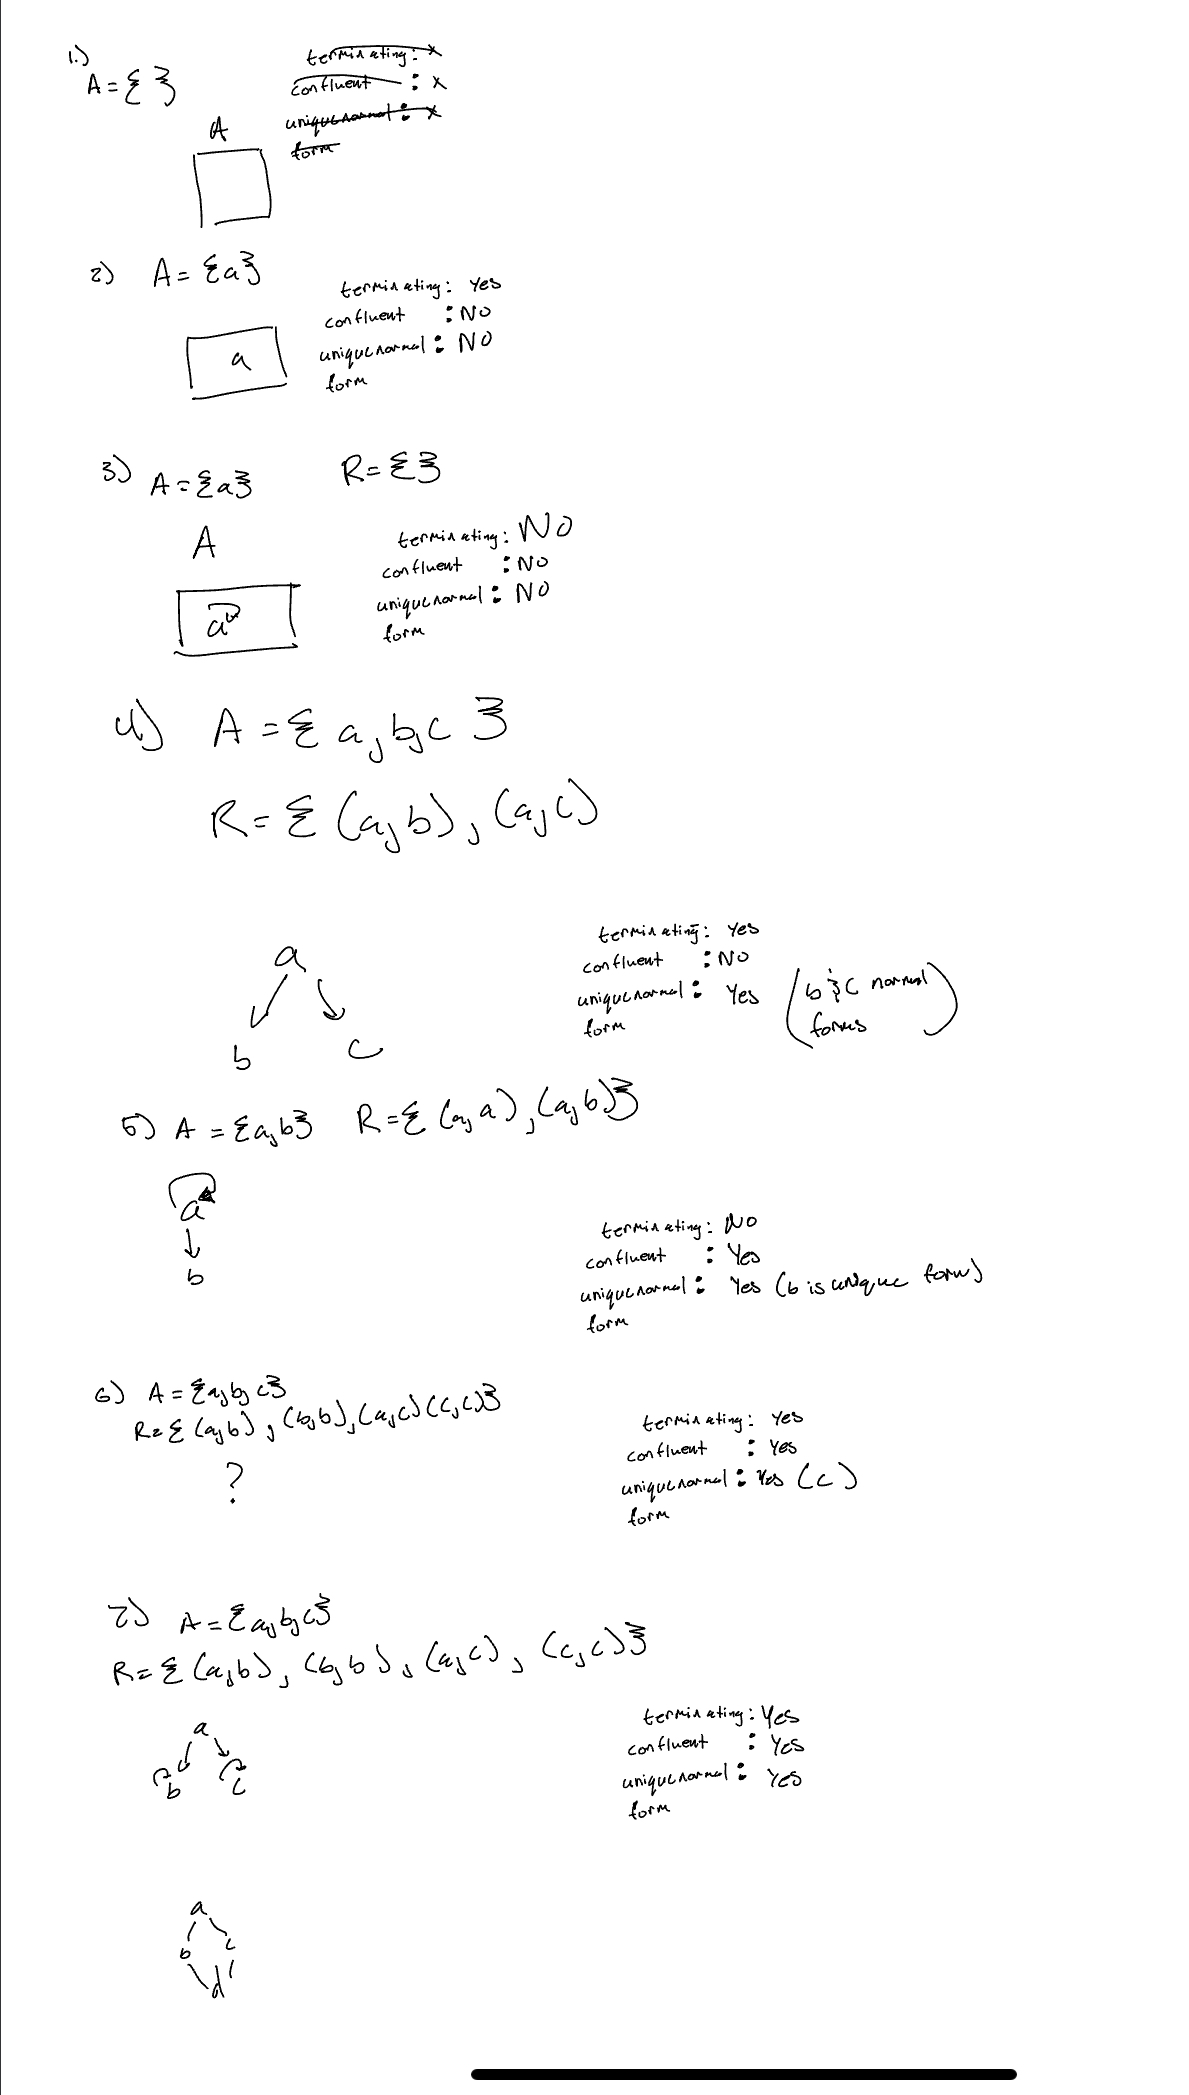
\includegraphics[scale=0.2]{hw7.jpg}
\subsection{Week 8}
 In week 8 we went over string rewriting exercises. We were shown how to analyze the ARS for each of given an algorithm by the professor.   
 \begin{enumerate}
\item Q) Why does the ARS not terminate?  A)The Ars does not terminate because the rules will reduce the left side lengths so it will end up reduced. 
\item Q) What are the normal forms? A)The normal forms would be “a, b” besides that I do not think there are normal forms unless I am misunderstanding.
\item Q)Can you change the rules so that the new ARS has unique normal forms (but still has the same equivalence relation)? A)Yes you can change the rules so that the new ARS has unique forms I believe we went over this class when we did and rewrote.  \begin{lstlisting} a a->  a
b b-> a
ab ->b
ba ->b \end{lstlisting}
\item Q) What do the normal forms mean? Describe the function implemented by the ARS. A)The normal forms can be used to identify the number of equivalence classes. The function would look like a for loop iterating and returning the sum/length.

   \end{enumerate}


\section{Project}\label{Project}
\subsection{Project Outline }
I was looking into having my project being more code and programming based since I am graduating soon and would like to have a project to put on my resume. I was really interested in making a webscrapping tool using haskell and scalpel but I think that might be a little too ambitious. But in terms of coding projects I am really interested in visual code like p5.js and processing. If there are any projects that involve creative and visual programming with haskell please let me know. Something like Perlin noise fields, 10PRINT, or even doing some ASCII art. But until I find something that I will be able to do like that I think I am going to try and make a program that does Mandelbrot sets in ASCII. I think that this is a achievable program that I could make in haskell. So I will be hopefully making graphical depiction of the Mandelbrot set. In the project I will be going over what Mandlebrot sets and how they can be graphically shown. Then I will be going into how it specifically works within haskell.

\section{Conclusions}\label{conclusions}

(approx 400 words)

In the conclusion, I want a critical reflection on the content of the course. Step back from the technical details. How does the course fit into the wider world of programming languages and software engineering?

\begin{thebibliography}{99}
\bibitem[PL]{PL} \href{https://github.com/alexhkurz/programming-languages-2022/blob/main/README.md}{Programming Languages 2022}, Chapman University, 2022.
\end{thebibliography}

\end{document}